% this file is called up by thesis.tex
% content in this file will be fed into the main document
\chapter{Σχεδιασμός στη Βάση Αρχειοθετημένης Γνώσης} % top level followed by section, subsection
%: ----------------------- paths to graphics ------------------------

% change according to folder and file names
\ifpdf
    \graphicspath{{3/figures/PNG/}{3/figures/PDF/}{2.5/figures/}}
\else
    \graphicspath{{3/figures/EPS/}{3/figures/}}
\fi

%: ----------------------- contents from here ------------------------
Σε αυτό το κεφαλαίο προτείνεται, υλοποιείται και αξιολογείται μια πρωτότυπη διαδικασία σχεδιασμού στροβιλομηχανών η οποία εκμεταλλεύεται τη διαθεσιμότητα  παλαιότερων αρχειοθετημένων σχεδιασμών. Οι τελευταίοι θεωρούνται βέλτιστοι ή πολύ ικανοποιητικοί για λειτουργία σε διαφορετικές μεν, αλλά «συναφείς» συνθήκες. Αυτή η διαδικασία θα ονομάζεται σχεδιασμός στη βάση αρχειοθετημένης γνώσης ή \english{Knowledge Based Design (KBD),} \cite{Kyriacou2010}. Αν και  το υλικό που παρουσιάζεται περιορίζεται σε περιπτώσεις στροβιλομηχανών, η μέθοδος είναι γενική και άμεσα εφαρμόσιμη σε οποιαδήποτε άλλη επιστημονική περιοχή.    

Η προτεινόμενη διαδικασία σχεδιασμού αποτελεί ένα πρωτότυπο συνδυασμό της γενικότερης μεθόδου «Αιτιολογίας Κατά Περίπτωση» \english{(Case Based Reasoning, CBR)}, \cite{kolodner_1991,slade_1991,riesbeck_1989}, που εντάσσεται στην κατηγορία «Συστημάτων Αρχειοθετημένης Γνώσης» \english{(Knowledge Based Systems, KBS)} και των ΕΑ. Η προτεινόμενη \english{KBD} αποτελεί μία εντελώς αυτοματοποιημένη διαδικασία, από τη στιγμή που έχουν επιλεγεί οι αρχειοθετημένοι σχεδιασμοί (σχεδιασμοί βάσης) και δεν απαιτεί παρέμβαση του χρήστη κατά τη διαδικασία αναθεώρησης της προτεινόμενης λύσης, όπως αυτό συμβαίνει στη συμβατική \english{CBR}. 
Το επιδιωκόμενο αποτέλεσμα θα μπορούσε, εν μέρει, να επιτευχθεί με απλή ένταξη των αρχειοθετημένων σχεδιασμών στην πρώτη γενιά του ΕΑ, μαζί με κατάλληλο καθορισμό των ορίων των μεταβλητών σχεδιασμού. Αντ' \newline αυτού, στην προτεινόμενη διαδικασία, χρησιμοποιούνται τεχνικές στατιστικής ανάλυσης έτσι ώστε να επιτευχθεί περαιτέρω επιτάχυνση του ΕΑ. Η προτεινόμενη διαδικασία \english{KBD} επιτυγχάνει:           

\begin{description}
  \item[α)] Αισθητή μείωση των μεταβλητών σχεδιασμού που χειρίζεται ο ΕΑ, επιφέροντας σημαντική επιτάχυνση της βελτιστοποίησης. Ουσιαστικά, επιτυγχάνει τον ε-ντοπισμό της/των βέλτιστης/ων λύσης/εων με μικρότερο αριθμό κλήσεων του λογισμικού αξιολόγησης. Επιπλέον, προκαλεί ακόμη μεγαλύτερη επιτάχυνση λόγω της αύξησης του κέρδους από τη χρήση μεταπροτύπων. Στην προτεινόμενη μέθοδο, τα μεταπρότυπα εκπαιδεύονται αποκτώντας μεγαλύτερη ακρίβεια πρόβλεψης ενώ η διαδικασία της ΠΠΑ μπορεί να εκκινεί νωρίτερα, με αρκετά λιγότερα πιθανά δείγματα εκπαίδευσης στη βάση δεδομένων την οποία διατηρεί και ανανεώνει ο ΕΑ, κατά την εξέλιξή του.   
  \item[β)] Τον αυτόματο/άκοπο καθορισμό των ορίων των μεταβλητών σχεδιασμού, απαλλάσσοντας έτσι το σχεδιαστή από τη διαδικασία επιλογής τους και εξαλείφο-ντας παράλληλα τον κίνδυνο λάθους (η βέλτιστη λύση να βρίσκεται έξω από τα όρια των μεταβλητών σχεδιασμού). Υπενθυμίζεται ότι η βελτιστοποίηση μέσω ΕΑ προαπαιτεί τον καθορισμό άνω και κάτω ορίων τιμών για κάθε μεταβλητή. 
    \item[γ)] Τη δυνατότητα αντιστοίχισης τιμών σημαντικότητας στις περιοχές του χώρου σχεδιασμού, όπως αυτές υπολογίζονται από τη στατιστική ανάλυση των αρχειοθετημένων σχεδιασμών. Η απόδοση υψηλής σημαντικότητας σε μια υποπεριοχή του χώρου σχεδιασμού μετουσιώνεται σε μεγαλύτερη πιθανότητα δημιουργίας απογόνων σε αυτήν, κατά τη διαδικασία της εξέλιξης.
\end{description}

Οι προαναφερθείσες ιδιότητες της \english{KBD} επιτρέπουν την αποδοτική ανίχνευση μεγάλων χώρων σχεδιασμού, τόσο ως πρός το πλήθος των μεταβλητών σχεδιασμού όσο και ως προς το εύρος αυτών,  εκμεταλλευόμενη την πληροφορία/γνώση που ενυπάρχει στους αρχειοθετημένους σχεδιασμούς.  


\section{Διατύπωση Νέου Σχεδιασμού}
Στην προτεινόμενη μέθοδο, ο τρόπος διατύπωσης κάθε νέου σχεδιασμού είναι άρρηκτα συνδεδεμένος με την εισαγωγή των λεγόμενων μεταβλητών βελτιστοποίησης (\english{optimization variables}). Οι μεταβλητές βελτιστοποίησης αποτελούν ένα διαφορετικό σύνολο μεταβλητών σχεδιασμού, μικρότερης κατά κανόνα διάστασης από αυτό που προκύπτει από την κλασική παραμετροποίηση μορφής. Στη μέθοδο \english{KBD}, οι άγνωστοι του προβλήματος θα ονομάζονται σκόπιμα «μεταβλητές βελτιστοποίησης»  για να υπάρξει αντιδιαστολή ως προς τις «μεταβλητές σχεδιασμού» που αντιστοιχούν στην κλασική παραμετροποίηση μορφής. Στην τελευταία περίπτωση, λ.χ. μεταβλητές σχεδιασμού θα μπορούσαν να είναι οι συντεταγμένες των σημείων ελέγχου συναρτήσεων \english{Bezier} κ.ο.κ.        

Η διαδικασία εισαγωγής των μεταβλητών βελτιστοποίησης έχει ως αφετηρία τους $m$ σχεδιασμούς βάσης ($m$ αρχειοθετημένα πτερύγια, αν λ.χ. σχεδιάζεται ένα νέο πτερύγιο στροβιλομηχανής). Αυτά θα συμβολίζονται ως $GEO_i=(x_1^i,x_2^i,....,x_N^i)$, $i\!=\!1,...,m$ όπου $x_j$, $j=1,...,N$ οι μεταβλητές σχεδιασμού όπως αυτές προκύπτουν από την παραμετροποίηση μορφής. Θεωρείται ότι οι $m$ σχεδιασμοί βάσης περιγράφο-νται όλοι με την ίδια παραμετροποίηση. Σε διαφορετική περίπτωση, επαφίεται στο σχεδιαστή να δημιουργήσει κοινή παραμετροποίηση. Αυτό μπορεί να γίνει λ.χ. μέσω ΕΑ αλλά το θέμα ξεφεύγει από το πλαίσιο της παρούσας διατριβής.     

Στη συνέχεια, υπολογίζονται οι μέσες τιμές ($\mu _j$) και οι τυπικές αποκλίσεις ($\sigma _j$) όλων των μεταβλητών σχεδιασμού των $m$ σχεδιασμών βάσης. Συμβολικά,
  
\begin{eqnarray}
		\left( {\begin{array}{c}
 		x_1^1  \\
 		\vdots  \\
 		x_N^1	\\
 		\end{array} } \right) 
 		\left( {\begin{array}{c}
 		x_1^i  \\
 		\vdots  \\
 		x_N^i	\\
 		\end{array} } \right)
 		\left( {\begin{array}{c}
 		x_1^m  \\
 		\vdots  \\
 		x_N^m	\\
 		\end{array} } \right) \rightarrow
		\left( {\begin{array}{c}
 		\mu _1  \\
 		\vdots  \\
 		\mu _N  \\
 		\end{array} } \right)
		\left( {\begin{array}{c}
 		\sigma _1  \\
 		\vdots  \\
 		\sigma _N  \\
 		\end{array} } \right)
   \label{cdf-matrix} 
\end{eqnarray}

Οι Ν μεταβλητές σχεδιασμού ομαδοποιούνται σε Κ ομάδες. Τα κριτήρια για την ομαδοποίηση μπορεί να είναι πολλά. Συνήθως, αλλά όχι αναγκαστικά, όλες οι μεταβλητές σχεδιασμού που αναφέρονται στην ίδια συνιστώσα της προς σχεδιασμό γεωμετρίας εντάσσονται στην ίδια ομάδα. Ενδεικτικά, κατά το σχεδιασμό λ.χ. μιας πτερύγωσης στροβιλομηχανής, οι μεταβλητές σχεδιασμού που παραμετροποιούν τη γενέτειρα του κελύφους ποδός συνήθως ανήκουν στην ίδια ομάδα, αυτές της γενέτειρας κελύφους κεφαλής σε μια άλλη, μια τρίτη ομάδα μπορεί να αποτελείται από τις μεταβλητές που σχετίζονται με τη μέση επιφάνεια κυρτότητας του πτερυγίου, κ.ο.κ. 

Στη σχέση που ακολουθεί εισάγονται συντελεστές βάρους $w_{i,k}$, όπου ο δεύτερος δείκτης αφορά στην ομάδα ($k=1,...,K$) στην οποία εντάχθηκε η αντίστοιχη μεταβλητή σχεδιασμού $x_j$. Κάθε νέος σχεδιασμός (άρα και ο ζητούμενος βέλτιστος) προκύπτει ως 

\begin{eqnarray}
   x_j^{new} = \Phi _j^{-1} (\frac{\sum_{i=1}^{m}w_{i,k} \Phi _j(x_j^i)}{\sum_{i=1}^{m}w_{i,k} }) 
   \label{non-linear2} 
\end{eqnarray}
όπου $\Phi_j$ η σιγμοειδής αθροιστική συνάρτηση κανονικής κατανομής για την $j$, δηλαδή η

\begin{eqnarray}
   \Phi _{j} (x)= \frac{1}{\sigma _j\sqrt[2]{2\pi}}\int _{-\infty}^x exp(\frac{-(u-\mu _j)^2}{2 \sigma _j^2 })du 
   \label{cdf} 
\end{eqnarray}
ενώ τα $\sigma _j$ και $\mu _j$ υπολογίζονται από τη σχέση \ref{cdf-matrix}. Στο σημείο αυτό αξίζει να τονισθεί η διάκριση στα χρησιμοποιούμενα σύμβολα. Υπενθυμίζεται ότι $x_j^i$ ($i=1,...,m$ και $j=1,...,N$) συμβολίστηκε η τιμή της $j$ μεταβλητής σχεδιασμού σύμφωνα με την παραμετροποίηση της  σχεδιαζόμενης μορφής για τον $i$-ιοστό σχεδιασμό βάσης. Αντι-θέτως, οι νέες μεταβλητές που θα χειριστεί ο ΕΑ («μεταβλητές βελτιστοποίησης») συμβολίζονται με $w_{i,k}$ και είναι $mK$ σε πλήθος. Σε αυτές, προστίθεται προαιρετικά μια ακόμη μεταβλητή, η $\Psi$.   
  
%Οι μεταβλητές βελτιστοποίησης που εισήχθησαν με αυτήν τη διαδικασία και τις οποίες τελικώς χειρίζεται ο ΕΑ, είναι τα βάρη ($w_{i,k}$, σχέση \ref{non-linear2}) τα οποία καθορίζουν τη συνεισφορά κάθε σχεδιασμού βάσης, ανάλογα με την ομάδα στην οποία εντάχθηκε η εκάστοτε μεταβλητή σχεδιασμού, στο νέο σχεδιασμό. Ο πρώτος δείκτης $(i)$, στο βάρος $w_{i,k}$, σχετίζεται με το σχεδιασμό βάσης και ο δεύτερος δείκτης $(k)$ με την ομάδα στην οποία ανήκει η $(j)$ μεταβλητή σχεδιασμού.      

Η προαιρετική μεταβλητή προεκβολής ($\Psi$) δίνει την επιπλέον δυνατότητα δημιουργίας νέων σχεδιασμών και εκτός του εύρους $\mu _j \pm 3\sigma _j$, \cite{Kiemele}. Χρησιμοποιώντας τη μεταβλητή αυτή, τα $\sigma _j$  (που υπολογίστηκαν από τη \ref{cdf-matrix}, τα οποία στη συνέχεια θα συμβολίζονται με $\sigma_j^{computed}$ για να διακρίνονται από τα τελικά $\sigma _j$ τα οποία θα  προκύψουν τελικά απο τη σχέση \ref{cdf-matrix-2})  υπολογίζονται από την          

\begin{eqnarray}
		\left( {\begin{array}{c}
 		\sigma _1  \\
 		\vdots  \\
 		\sigma _N  \\
 		\end{array} } \right) =
 		\Psi  
 		\left( {\begin{array}{c}
 		\sigma _1^{computed}  \\
 		\vdots  \\
 		\sigma _N^{computed}  \\
 		\end{array} } \right)
   \label{cdf-matrix-2} 
\end{eqnarray}
και είναι αυτά που θα χρησιμοποιηθούν για το σχηματισμό των νέων σχεδιασμών. 

Ο αριθμός των μεταβλητών βελτιστοποίησης που προκύπτει, ισούται με $m K+1$, συνυπολογίζοντας και την προαιρετική μεταβλητή  $\Psi$.


\section{Εφαρμογή: Σχεδιασμός 2Δ πτερύγωσης συμπιεστή}
\label{Drela1}
Η προτεινόμενη μέθοδος πιστοποιείται στο σχεδιασμό της αεροτομής 2Δ πτερύγωσης συμπιεστή. Η πτερύγωση λειτουργεί σε αριθμό \english{Mach} εισόδου $M_1=0.54$, γωνία εισόδου ροής$a_1=44^o$ και αριθμό \english{Reynolds} της ροής βασισμένο στη χορδή $c$ ίσο με $Re=4\times10^5$. Στόχος της βελτιστοποίησης είναι η ελαχιστοποίηση των απωλειών ολικής πίεσης $P_t$, στη μορφή του ομώνυμου συντελεστή   
\begin{eqnarray}
   \omega=\frac{p_{t1}-p_{t2}}{p_{t1}-p_1}
   \label{omegaLosses} 
\end{eqnarray}
όπου ο δείκτης $1$ υποδηλώνει την είσοδο ενώ ο δείκτης $2$ την έξοδο της πτερύγωσης.

Η προς σχεδιασμό αεροτομή υπόκειται σε γεωμετρικούς περιορισμούς που αφορούν στο ελάχιστο επιτρεπόμενο πάχος της σε διάφορες θέσεις. Στις θέσεις  $0.3c$, $0.6c$ και $0.9c$, όπου $c$ είναι το μήκος της αεροτομής, το ελάχιστο επιτρεπτό πάχος της αεροτομής είναι $0.10c$, $0.08c$ και $0.01c$, αντίστοιχα. Επίσης, η προς σχεδιασμό αεροτομή απαιτείται να προκαλεί στροφή της ροής $\Delta a= |a_2-a_1|$ μεγαλύτερη των $30^o$. Η παραμετροποίηση υλοποιείται χωριστά για τη μέση γραμμή κυρτότητας και την κατανομή πάχους και χρησιμοποιεί $27$ μεταβλητές σχεδιασμού. Κατά τον επιχειρούμενο με \english{KBD} σχεδιασμό, το διάνυσμα μεταβλητών σχεδιασμού χωρίζεται σε τρεις ομάδες ($K=3$) ως εξής: \english{i}) αυτές που ελέγχουν το σχήμα της μέσης γραμμής κυρτότητας \english{ii}) αυτές που ελέγχουν την κατανομή πάχους στην πλευρά υπερπίεσης και \english{iii}) αυτές που ελέγχουν την κατανομή πάχους στην πλευρά υποπίεσης. Στη διάθεσή του σχεδιαστή υπάρχουν $m=4$ αρχειοθετημένοι σχεδιασμοί που χρησιμοποιούνται ως γεωμετρίες βάσης. Τελικώς, οι μεταβλητές βελτιστοποίησης είναι $m K+1=13$ και αυτές, αντί των $27$, χειρίζεται ο ΕΑ. Λογισμικό αξιολόγησης είναι μια ολοκληρωματική μέθοδος επίλυσης των συνεκτικών στρωμάτων, σε συνδυασμό με επιλύτη των εξισώσεων \english{Euler} για την εξωτερική ροή, \cite{Drel1987}.          

Οι επιδόσεις των $m\!=\!4$ σχεδιασμών βάσης (σχήμα \ref{CBRarch}) στις επιθυμητές συνθήκες ροής μαζί με την προκαλούμενη στροφή της ροής έχουν ως εξής:  
\begin{itemize}
\item{Σχεδιασμός βάσης $Β_1$:} $\omega=0.0207$ και $\Delta a=36.3^o$.
\item{Σχεδιασμός βάσης $Β_2$:} $\omega=0.0278$ και $\Delta a=27.8^o$.
\item{Σχεδιασμός βάσης $Β_3$:} $\omega=0.0201$ και $\Delta a=37.5^o$.
\item{Σχεδιασμός βάσης $Β_4$:} $\omega=0.0237$ και $\Delta a=33.1^o$.
\end{itemize}
 
\begin{figure}[h!]
\begin{minipage}[b]{1\linewidth}
 \centering
 \resizebox*{14cm}{!}{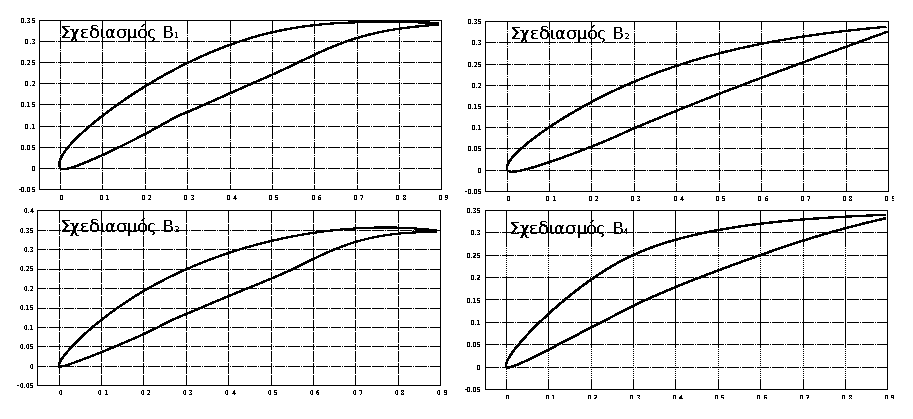
\includegraphics{blade_s.eps}}
\end{minipage}
\caption{Σχεδιασμός 2Δ πτέρυγωσης συμπιεστή: Οι $4$ αεροτομές που  χρησιμοποιήθηκαν ως σχεδιασμοί βάσης κατά την εφαρμογή της μεθόδου \english{KBD}, τοποθετημένες στην επιθυμητή γωνία κλίσης της πτερύγωσης.} 
\label{CBRarch}
\end{figure}

Παρατηρείται ότι και οι $4$ σχεδιασμοί βάσης, όταν χρησιμοποιηθούν στις επιθυμητές συνθήκες ροής αντί των συνθηκών για της οποίες είχαν σχεδιαστή (περιγράφο-νται στο πλήρες κείμενο), έχουν σχετικά μεγάλες τιμές απωλειών $\omega$. Επιπροσθέτως, ο σχεδιασμός β, δεν σέβεται τον περιορισμό στροφής της ροής. Και οι $4$ σχεδιασμοί βάσης σέβονται, από σύμπτωση ενδεχομένως, τους γεωμετρικούς περιορισμούς.    

Για τη μελέτη των επιδράσεων που έχει η χρήση της μεθόδου \english{KBD} τόσο στην εξέλιξη αυτή καθαυτή όσο και στη χρήση μεταπροτύπων κατά τη διαδικασία της βελτιστοποίησης, πραγματοποιήθηκαν $4$ ξεχωριστές διαδικασίες βελτιστοποίησης. Η πρώτη έκανε χρήση του κλασικού ΕΑ, η δεύτερη ενός ΕΑ υποβοηθούμενου από μεταπρότυπα (\english{MAEA}), η τρίτη ενός ΕΑ με \english{KBD} (\english{KBD-EA}) και, τέλος, η τέταρτη ενός \english{MAEA} με \english{KBD} (\english{KBD-MAEA}). Λεπτομερής περιγραφή των παραμέτρων εξέλιξης που χρησιμοποιήθηκαν υπάρχει στο πλήρες κείμενο της διατριβής, στο α-ντίστοιχο κεφάλαιο. Είναι όμως σημαντικό να αναφερθεί ότι οι $27$ μεταβλητές σχεδιασμού που χρησιμοποιήθηκαν στις δύο πρώτες μεθόδους, σύμφωνα με την παραμετροποίηση της γεωμετρίας με \english{NURBS}, έδωσαν τη θέση τους σε μόνο $13$ μεταβλητές βελτιστοποίησης κατά την εφαρμογή των δύο τελευταίων.   
Οι πορείες σύγκλισης των προαναφερθεισών διαδικασιών βελτιστοποίησης συγκεντρώνονται στο σχήμα \ref{CBRDrela}.           

\begin{figure}[h!]
\begin{minipage}[b]{1\linewidth}
 \centering
 \resizebox*{11cm}{!}{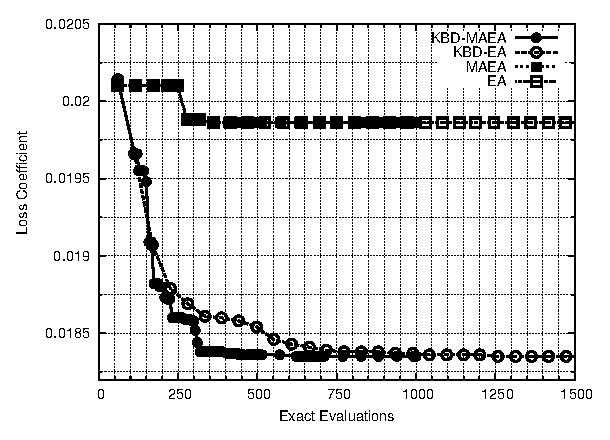
\includegraphics{Comp.eps}}
\end{minipage}
\caption{Σχεδιασμός 2Δ πτέρυγωσης συμπιεστή: Πορείες σύγκλισης των  ΕΑ, \english{MAEA}, \english{KBD-EA} και \english{KBD-MAEA}. Ο οριζόντιος άξονας αντιστοιχεί σε κλήσεις στο λογισμικό ΥΡΔ. Η εκπαίδευση των μεταπροτύπων έχει μηδενικό πρόσθετο κόστος. } 
\label{CBRDrela}
\end{figure}

Παρατηρείται ότι η χρήση μεταπροτύπων στον ΕΑ (ή ΜΑΕΑ) χωρίς επιπρόσθετη χρήση \english{KBD} δεν απέφερε κέρδος. Αυτό, κατά μεγάλο βαθμό, οφείλεται στο σχετικά πολύ μεγάλο εύρος του χώρου σχεδιασμού. Ακόμη, παρατηρείται η καθολική υπεροχή της μεθόδου \english{KBD-EA} συγκριτικά με τον κλασικό ΕΑ, αποδεικνύοντας έτσι την επιτάχυνση της εξέλιξης όταν χρησιμοποιούνται οι νέες μεταβλητές βελτιστοποίησης (μειωμένος αριθμός και εισαγωγή σημαντικότητας στις περιοχές του χώρου σχεδιασμού). Επίσης, παρατηρείται η επανεμφάνιση του «απωλεσθέντος» κέρδους λόγω της χρήσης μεταπροτύπων κατά τη διαδικασία της ΠΠΑ στον \english{KBD-MAEA}. Τα παραπάνω συνηγορούν στην αξία της μεθόδου \english{KBD}, είτε αυτή χρησιμοποιείται μαζί με τον ΕΑ ή το ΜΑΕΑ.            

Η βέλτιστη αεροτομή που υπολογίστηκε από τον \english{KBD-MAEA} παρουσιάζεται στο σχήμα \ref{CBRDrelaRes}. Έχει απώλειες ολικής πίεσης $\omega=0.01834$, τιμή αρκετά μικρότερη από όλους τους σχεδιασμούς βάσης. Επίσης ικανοποιεί όλους  του περιορισμούς και επιφέρει στροφή της ροής ίση με $\Delta a = 30.2^o$. 
%The optimal blade resulting form KBD-MAEA is presented in fig. \ref{CBRDrelaRes}. The design delivers $\omega=0.01834$ and $\Delta a = 30.2^o$ at the desirable conditions. The design is better than all basis design (operating at the desirable conditions) and respects all the constraints. The delivered form KBD-MAEA design is also of significantly better quality than the designs delivered by all the non-KBD optimization procedures. 


\begin{figure}[h!]
\begin{minipage}[b]{1\linewidth}
 \centering
 \resizebox*{14cm}{!}{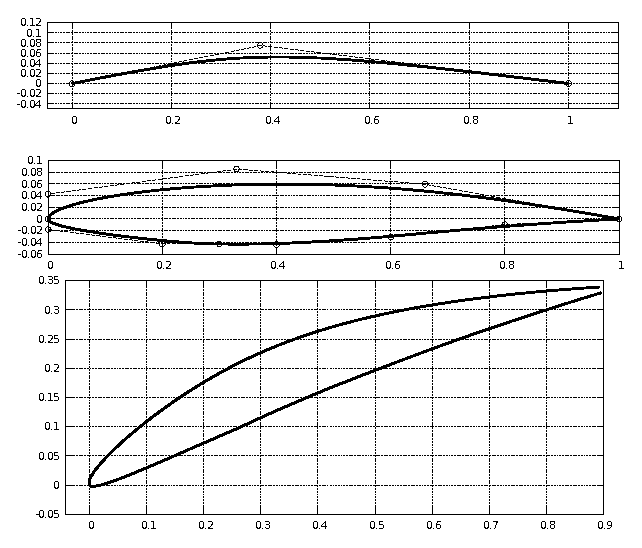
\includegraphics{ResD1.eps}}
\end{minipage}
\caption{Σχεδιασμός 2Δ πτέρυγωσης συμπιεστή: Η βέλτιστη αεροτομή η οποία υπολογίστηκε από τη μέθοδο \english{KBD-MAEA}. Η μέση γραμμή (πάνω) και οι κατανομές πάχους (κέντρο) για τις πλευρές υπερπίεσης και υποπίεσης, μαζί με τα πολύγωνα ελέγχου των πολυωνύμων \english{NURBS} που τις παρήγαγαν. Η βέλτιστη αεροτομή, τοποθετημένη στην επιθυμητή γωνία κλίσης της πτερύγωσης (κάτω). Η αεροτομή ικανοποιεί όλους τους τεθέντες περιορισμούς.} 
\label{CBRDrelaRes}
\end{figure}

%\begin{figure}[h!]
%\begin{minipage}[b]{1\linewidth}
% \centering
% \resizebox*{12cm}{!}{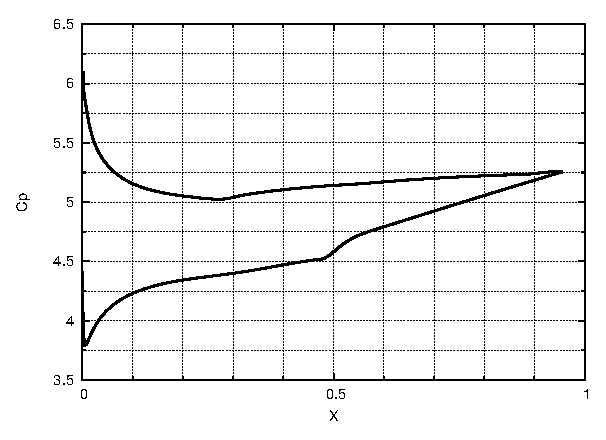
\includegraphics{Best_CP.eps}}
%\end{minipage}
%\caption{Συντελεστή πίεσης $C_p$ για την βέλτιστη αεροτομή της %εικόνας \ref{CBRDrelaRes}.} 
%\label{CBRDrelaRes_cp}
%\end{figure}


%
% ---------------------------------------------------------------------------
% ----------------------- end of thesis sub-document ------------------------
% ---------------------------------------------------------------------------
